% Introduction
% ============

\chapter{Introduction}
\label{ch:introduction}

\section{Qu'est-ce que la calculabilité ?}
\label{sec:qu_est-ce_la_calculabilite}

La calculabilité est l'étude des limites de l'informatique. C'est un domaine important de l'informatique qui permet de comprendre, d'analyser et d'appliquer ces limites.
Il faut savoir différencier les limites théoriques des limites
pratiques. La calculabilité est un domaine d'étude qui s'intéresse aux limites théoriques alors que
la complexité s'occupe des limites pratiques. Cette dernière
détermine la frontière entre ce qui est faisable et infaisable en pratique.
La question principale de la calculabilité est: \og quels sont les \textit{problèmes} qui (ne) peuvent (pas)
être résolus par un \textit{programme} ?\fg.  De manière informelle, un problème est dit \emph{calculable} s'il existe un programme qui résout ce problème.  La caractéristique d'un problème calculable ne donne donc aucune
autre information que la preuve de l'existence d'un programme capable de résoudre ce problème. On peut reformuler la notion de calculabilité comme : Si un algo existe, alors il y a peut-être une chance afin de pouvoir l'écrire pour résoudre le problème.  Mais lorsqu'un problème est non calculable, cela nous informe qu'il est inutile d'essayer d'écrire un programme pour résoudre ce problème; un tel programme n'existe pas!
La notion de calculabilité est donc importante à maitriser et peut-être très utile en entreprise par exemple. Si votre employeur vous demande de résoudre un problème non-calculable, il faut être capable de lui dire que c'est tout simplement impossible à faire pour ne pas perdre son temps.

\paragraph{} Le but est donc de tracer des frontières entre les programmes calculables,
non calculables et non calculables en pratique.

\subsection{Exemples de limites}
\label{subsec:exemples_limites}

De nombreuses limites existent en informatique. Par exemple, il est impossible de déterminer lorsqu'un programme se termine (cfr. Théorème de Rice \ref{sub:theoreme_de_rice}), de déterminer si un programme est écrit sans bugs ou encore d'écrire un programme sachant déterminer si deux programmes sont équivalents.

Mais des limites théoriques existent aussi dans des domaines scientifiques autres que l'informatique.

En physique par exemple, les lois de la thermodynamique établissent le fait que l'on ne peut créer de l'énergie à partir de rien (principe de Lavoisier notamment). Dans un autre registre, on sait qu'il est impossible d'observer, avec la précision que l'on souhaite, en même temps la \textit{position} et la \textit{vitesse} d'un électron.

En mécanique, on sait qu'il est impossible de construire une machine réalisant un mouvement perpétuel.

En mathématique, il est impossible de trouver deux nombres entiers $m$ et $n$ tels que $m^2 = 2n^2$, ou de trouver une fraction $\frac{m}{n}$ exprimant le rapport entre le rayon d'un cercle et sa circonférence, ou encore de diviser un angle en trois parties égales en utilisant uniquement une règle et un compas.

\section{Notion de problème}
\label{sec:notion_de_probleme}

Premièrement, on doit parler de la notion de problème.
Attention, il ne faut pas confondre un problème avec un programme.
Les caractéristiques d'un problème sont :

\begin{itemize}
	\item un problème est \emph{générique}: il s'applique à un ensemble de données ;
	\item pour chaque donnée particulière, il existe une réponse.
\end{itemize}

On représente un problème dans le cours par une fonction (noté $\phi$ ou $\varphi$).
Un problème est une spécification où j'ai un input et je veux un output.
La description d'un problème est donc équivalente à la description d'une fonction.

\paragraph{Exemples de problèmes}
\begin{itemize}
	\item additionner deux entiers ;
	\item étant donné une liste d'étudiants et de leurs points d'examen, trouver les étudiants dont la moyenne des examens est supérieure ou égale à $12/20$ ;
	\item déterminer si un polynôme à coefficients entiers a des racines entières.
\end{itemize}

\section{Notion de programme}
\label{sec:notion_de_programme}

Un programme (ou algorithme) est une \og procédure effective\fg, c'est-à-dire exécutable par une machine. Par exemple un programme java.\\

La compréhension du concept de programme est basée sur la compréhension du concept de \og programme écrit dans un langage de programmation\fg.\\

Il existe plein de formalismes permettant la description d'une \og procédure effective\fg.

\section{Qu'est-ce que la complexité ?}
On a vu à quoi servait la calculabilité et que ce concept est assez abstrait. D'un autre côté, nous avons la complexité qui aborde des concepts plus concrets. Elle se demande quelles sont les ressources : le temps, l'espace mémoire, etc. mis en oeuvre pour résoudre le problème.
Elle étudie l'efficacité d'un programme. La définition d'efficacité est la suivante : mesure des ressources nécessaires à mettre en oeuvre pour que le programme produise les résultats attendus.
Il est important de noter qu'on veut développer des concepts de complexité qui soient totalement indépendants des nouvelles technologies, de la machine utilisée et encore du formalisme utilisé.
En très grande lignes, la complexité est la limite entre l'infaisable en pratique et le faisable en pratique. 


\section{Résultats principaux}
\label{sec:r_sultat_principaux}

\subsection{Équivalence des langages de programmation}
\label{subsec:equivalence_des_langages_de_programmation}

Existe-t-il des langages de programmation plus puissants que d'autres? Tous les langages sont-ils équivalents?

Il y a une équivalence entre langages en termes de calculabilité.  Lorsqu'un problème est résolvable par un de ces langages, alors il l'est également par les autres.
S'il existe un programme \java qui résout un problème, il existera aussi un programme C/C++, PHP,\ldots{} qui peut résoudre le même problème. Il s'agit d'une équivalence théorique.

D'un point de vue théorique ces langages s'appellent des \emph{langages complets}. Ils permettent tous de résoudre les mêmes problèmes. Un problème est donc calculable indépendamment du langage utilisé.

D'un point de vue pratique on peut voir des différences (le programme est plus court, ou s'écrit plus rapidement, ou s'exécute plus rapidement, ou est plus propre, ou plus fiable, etc). Certains langages sont donc mieux adaptés que d'autres pour certaines classes de problèmes.


\subsection{Existence de problèmes non calculables}
\label{subsec:existence_de_problemes_non_calculables}
	Il existe des problèmes qui ne peuvent être résolus par un programme et qui sont alors dit \emph{non calculables}.
	Quelques exemples:
	\begin{itemize}
		\item détection de virus ;
		\item équivalence de programme ;
		\item déterminer si un polynôme à coefficients entiers a des racines entières, \ldots
	\end{itemize}
% section r_sultat_principaux (end)

\subsubsection{Exemple: Détection de virus informatique}
\label{subsubsec:detection_de_virus_informatique}
On veut déterminer si un programme \lstinline|P| avec une entrée \lstinline|D| est nuisible.

\begin{mydef}
	Un programme est dit \emph{nuisible} si son exécution a pour effet de contaminer d'autres programmes (par exemple en se recopiant autre part). Dans certains cas, il peut également être considéré comme dangereux lorsqu'il rend la machine partiellement ou totalement inutilisable (par exemple un cheval de Troie contenant une bombe logique ou une fork bomb).
\end{mydef}

Un bon antivirus serait alors un programme qui testerait des programmes en regardant s'ils se multiplient, tout en les empêchant de modifier (voir d'endommager) d'autres fichiers. Un tel programme, s'il existe, serait du même type que \lstinline|détecteur(P, D)| avec \lstinline|P| le programme à détecter et \lstinline|D| un état du système de données dans lequel le programme s'exécuterait.

\noindent Spécification du programme \lstinline|détecteur(P, D)|:\\
\textbf{Préconditions:} un programme \lstinline|P| et une donnée \lstinline|D|\\
\textbf{Postconditions:} \lstinline|"Mauvais"| si \lstinline|P(D)| est nuisible, \lstinline|"Bon"| sinon.

\begin{center}
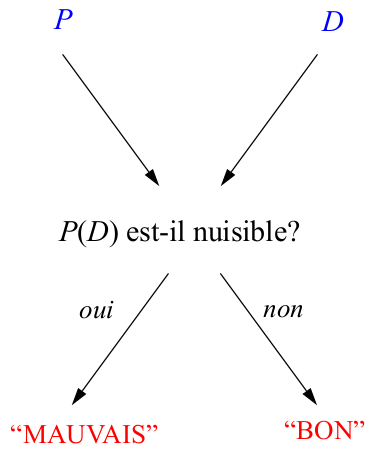
\includegraphics[scale=0.45]{Images/effet_detecteur.png}
\end{center}

Cependant il faut aussi que le détecteur ne soit pas nuisible pour que cette spécification soit valide. Or comme nous allons le démontrer, le détecteur ne peut être non nuisible.

\begin{mytheo}
	Il n'est pas possible d'écrire un programme antivirus non nuisible
	qui puisse déterminer avec sûreté
	si un programme \lstinline|P| est nuisible avec une entrée \lstinline|D|.
\end{mytheo}
\begin{proof}
Pour le prouver nous allons émettre l'hypothèse qu'un programme \lstinline|détecteur(P, D)| existe et qu'il n'est pas nuisible. Dans ce cas, nous pouvons construire le programme \lstinline|drôle(P)| suivant :

\label{lst:detecteur_de_virus}
\begin{lstlisting}
drôle(P)
    if détecteur(P,P) = "Mauvais"
        then stop
    else infecter un autre programme en y insérant P
\end{lstlisting}

Regardons maintenant si l'exécution de \lstinline|drôle(drôle)|, c'est-à-dire si l'on donne le code source de \lstinline|drôle| à lui-même, est nuisible ou non.
\begin{lstlisting}
drôle(drôle)
    if détecteur(drôle, drôle) = "Mauvais"
	    then stop
    else infecter un autre programme en y insérant drôle
\end{lstlisting}

\begin{center}
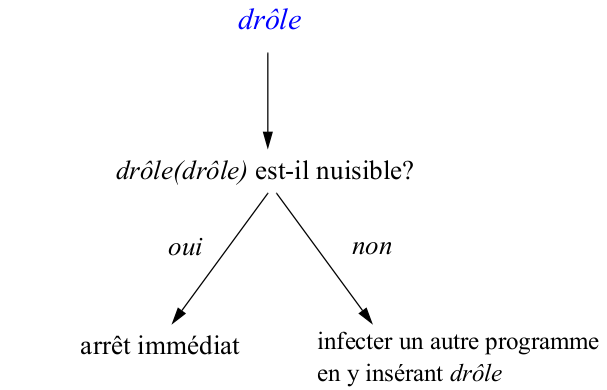
\includegraphics[scale=0.5]{Images/drole_de_drole.png}
\end{center}

\begin{itemize}
	\item Supposons que \lstinline|drôle(drôle)| soit nuisible.
      Lorsqu'on exécute, \lstinline|drôle(drôle)|,
      \lstinline|détecteur(drôle,drôle)| n'infecte rien car \lstinline|détecteur| n'est pas nuisible.

      Comme \lstinline|détecteur| retourne \lstinline|"Mauvais"|,
      le programme s'arrête.
      Rien n'a donc été infecté, ce qui est contradictoire avec le fait que \lstinline|drôle(drôle)| soit nuisible.
	\item Si par contre il n'est pas nuisible, alors \lstinline|détecteur(drôle,drôle)|
      ne va pas retourner \lstinline|"Mauvais"| et le code de la clause \lstinline|else| s'exécutera.
      Un autre programme est alors infecté ce qui contredit le fait que \lstinline|drôle(drôle)| ne soit pas nuisible.
\end{itemize}

On a donc une contradiction dans tous les cas, ce qui implique que le programme \lstinline|drôle| ne peut pas
exister. Vu que la seule hypothèse que nous avons formulée pour écrire le programme \lstinline|drôle| soit que le programme \lstinline|détecteur| (non nuisible) existe,
le programme \lstinline|détecteur| (non nuisible) ne peut pas exister non plus.
\end{proof}
% subsubsection d_tection_de_virus (end)

\subsection{Existence de problèmes intrinsèquement complexes}
\label{subsec:existence_de_problemes_intrinsequement_complexes}

\begin{mydef}
	Un problème \emph{intrinsèquement complexe} est un problème dont le meilleur algorithme n'a pas une complexité polynomiale, mais une complexité exponentielle ou pire. Peu importe les évolutions technologiques, un problème exponentiel ne peut et ne pourra être résolu que pour des données de petites tailles.  Un exemple est le problème du voyageur de commerce qui doit rechercher le trajet le plus court pour relier $n$ villes. Pour un problème intrinsèquement complexe, lorsqu'un ordinateur est $n$ fois plus rapide, la taille des problèmes pouvant être résolus en temps raisonnable est incrémentée d'une petite valeur (voir le tableau ci-dessous).
\end{mydef}

Supposons un ordinateur actuel sachant faire 100 millions d'instructions par secondes ($100$ Mips) et que le traitement d'un élément nécessite 100 instructions machines. Dénotons $N_i$  la taille du \og plus grand\fg{} exemple dont la solution peut-être calculée en 1 heure de temps calcul.

\begin{center}
	$\begin{array}{|c||c|c|c|}
		\hline
		\text{Complexité} & \text{Ordinateur actuel} & \text{100x plus rapide} & \text{1000x plus rapide} \\
		\hline
		n & N_1 = 3.6\times 10^9 & 100 N_1 & 1000 N_1 \\
		n^2 & N_2 = 6\times 10^5 & 10 N_2 & 31.6 N_2 \\
		n^3 & N_3 = 1530 & 4.64 N_3 & 10 N_3 \\
		n^5 & N_4 = 81 & 2.5 N_4 & 3.98 N_4 \\
		\hline
		2^n & N_5 = 31 & N_5 + 6 & N_5 + 10 \\
		3^n & N_6 = 20 & N_6 + 4 & N_6 + 6 \\
		\hline
	\end{array}$
\end{center}

Ce tableau montre dès lors que, peu importe les évolutions technologiques, un problème intrinsèquement complexe \textbf{ne peut} et \textbf{ne pourra} être résolu que pour de petits exemples.

Cependant, dans la pratique, certains algorithmes résolvent efficacement les problèmes pratiques, et d'autres, également efficaces, permettent d'obtenir des \textbf{approximations} des solutions exactes.

De manière générale, un problème intrinsèquement complexe est un problème possible à résoudre de manière théorique mais qui en pratique demande trop de ressources et sa résolution devient donc impossible.
\section{Objectifs calculabilité et complexité}
\label{sec:objectifs_calculabilite_et_complexite}

La Figure~\ref{cal_non_cal} illustre la frontière entre les problèmes non calculables (il n'existe pas un programme capable de répondre à la question) et calculables (il existe un programme capable de répondre à la question) dans l'univers des problèmes. Parmi les problèmes calculables, il y a ceux qui le sont en pratique (pas exponentiels) et ceux qui ne sont pas calculables en pratique.
\begin{figure}[h]
	\centering
	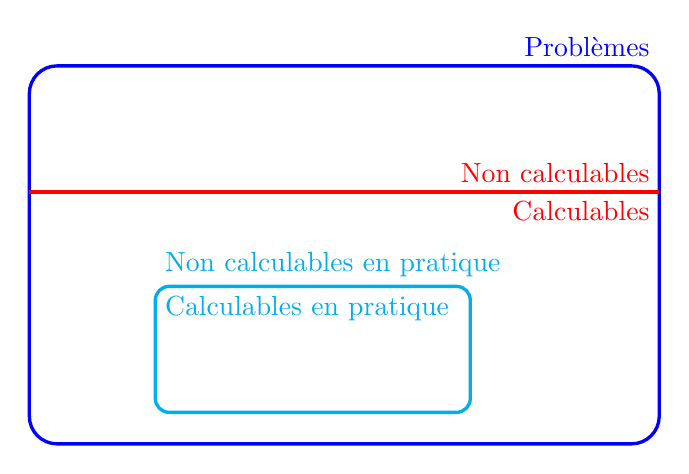
\begin{tikzpicture}[scale=0.8]
	\draw[very thick,blue,rounded corners=10pt]  (0,0) rectangle (10,6);
	\draw[very thick,red]   (0,4) -- (10,4);
	\draw[very thick,cyan,rounded corners=5pt] (2,0.5) rectangle (7,2.5);
	\draw[blue]  (10,6)  node[above left] {Problèmes};
	\draw[red]   (10,4)  node[above left] {Non calculables};
	\draw[red]   (10,4)  node[below left] {Calculables};
	\draw[cyan] (2,2.5) node[above right] {Non calculables en pratique};
	\draw[cyan] (2,2.5) node[below right] {Calculables en pratique};
	\end{tikzpicture}
	\caption{Problèmes calculables / non calculables}
	\label{cal_non_cal}
\end{figure}

L'intérêt de la calculabilité est de savoir quels problèmes sont calculables ou lesquels ne le sont pas. Si un problème est non calculable, il est alors inutile  d'essayer de résoudre ce problème.  Si le problème est calculable mais intrinsèquement complexe, il est inutile d'envisager un algorithme permettant de résoudre des problèmes de grande taille.
Face à un problème non calculable ou intrinsèquement complexe, on peut essayer de relâcher le problème pour le rendre calculable ou de complexité polynomiale. Une solution à ce problème relâché peut par exemple être une approximation du problème initial.
% section introduction (end)Introduction

